\documentclass[11pt,a4paper]{report}
\usepackage[latin1]{inputenc}
\usepackage{amsmath}
\usepackage{amsfonts}
\usepackage{amssymb}
\usepackage{graphicx}
\usepackage[left=3.00cm]{geometry}
\usepackage{helvet} %uarial alt. package for arial font! Try to see if its better
\usepackage{natbib} %https://www.sharelatex.com/learn/Natbib_citation_styles
\renewcommand{\familydefault}{\sfdefault}

\title{Enhancing Social HRI using Affective Communication}
\author{Katie Winkle}
\begin{document}
\maketitle

\section{Abstract}

\section{Acknowledgements}

\tableofcontents

\chapter{Introduction}
[intro]
[background/motivation]
[aims/objectives, remember feedback that these can be quite specific now -> high level hypotheses]
[after reading this reader should know premise and context of final experiment so can refer to it before explaining in detail in methodology section]

\chapter{Literature Review}
[intro paragraph]
\section{IET and Emotional Expression in Humans}

\subsection{IET and its Impact on Human Behaviour}
There are different hypotheses concerning the purpose of IET and emotional expression more generally in HHI. A functionalist approach (considering the consequences in order to determine the purpose) suggests that at the dyadic level, emotion expressions help individuals determine other's emotions, beliefs, intentions and orientation towards their relationship; and that evoking emotions in others is associated with behaviours such as avoidance, helping, affiliation and soothing \cite{keltner1999social}. An evolutionary approach (considering development over time and the link to population fitness) suggests that emotional expression evolved from being a physiological response (e.g. scrunching the nose to prevent inhalation of noxious gas) into a form of social communication, which observers evolved an ability to instantly and subconsciously decode in order to obtain information about the expresser and/or their environment \cite{shariff2011emotion}. Regardless of exact purpose, a consistent theme in psychology literature is the importance and subconscious nature of IET resulting from emotional expression in communication, and this is what has the greatest relevance to HRI. 

There is evidence to suggest that one form of IET is social appraisal, whereby individual human judgement is influenced by the perceived judgement of others \cite{parkinson2011interpersonal}. Specifically, it has been demonstrated that judgement of an everyday object differs depending on whether it is presented alongside a smiling or disgusted face \cite{bayliss2007affective} suggesting that emotional expression is a trigger for this form of IET. Another experiment demonstrated that even in a very dangerous situation (a simulated fire) participants surrounded by seemingly calm and unresponsive actors were slower to react than participants that were alone; it has been argued that this could be due to IET effects whereby the participants felt calmer due to the calmness of the actors and also judged the situation to be less dangerous based on their perceived lack of concern (\cite{latane1968group} as discussed in \cite{parkinson2011interpersonal}).

Another evidenced form of IET is emotion contagion, whereby an individual's emotional state changes based on that of their interaction partner; however, this is less well understood and more difficult to experimentally examine than social appraisal effects \cite{parkinson2011interpersonal}. There is a general consensus that most emotion contagion is a form of social mimicry, however, it is disputed whether this is based on physical mimicry, in which the related emotion is generated from mimicking the physical expression; i.e. the individual smiles in response to a smile and hence feels happier \cite{strack1988inhibiting}, or whether expression is less important and actually an individual must understand and perceive the reason for another's emotional expression in order for emotion contagion to occur \cite{tamietto2009unseen}. In contrast to the idea of simple mimicry it should also be noted that emotion contagion has been demonstrated to induce contrasting rather than matching emotions, and that this may be linked to social stature \cite{tiedens2003power}.

Demonstrated examples of emotion contagion highlight the impact it can have both at the individual and group level. For example, listening to neutral information spoken in an emotional way can induce similar emotions in the listener \cite{neumann2000mood}, and emotion contagion in a group can improve attitudes and reduce conflicts resulting in improved task performance \cite{barsade2002ripple}. It has even been demonstrated that emotion contagion can occur through social networks, with Facebook users producing more positive or negative posts when the amount of negative or positive emotional content in their newsfeed was reduced respectively \cite{kramer2014experimental}. Other interesting results include thirsty individuals pouring more or less from a drink jug if exposed to a smiling or frowning face respectively \cite{winkielman2005unconscious} or acceptance of an offer being higher for smiling and lower for frowning proposers compared to those that wore neutral expressions \cite{mussel2013value}. 

As such, whilst the origins and exact mechanisms of IET are not clear, the evidence presented suggests it has significant impact on HHI and can influence an individual's feelings, judgement and behaviour as well as group collaboration and effectiveness. This warrants the study of IET in HRI in order to establish whether the same effects can be observed, and if so whether they can be useful e.g. in improving things like robot effectiveness and acceptance or task performance. Key research questions include whether robot to human IET can occur and how robot emotional expressions affect human judgements and behaviour. Additionally, the number of unconfirmed hypothesise in the psychology literature suggests that HRI experiments dealing with emotion in a very controlled way might be useful as a mechanism for testing theories and contributing to psychological understanding of the role of human emotions. 


\subsection{Human Displays of Emotion}
In order to design emotionally expressive robot behaviours it must first be established how emotion is expressed in humans and identify specific behaviours which might be transferable onto a robot. Specifically the robotic platform to be used for this project is Aldebaran Robotics' humanoid robot NAO\footnote{https://www.aldebaran.com/en/cool-robots/nao}, which means that facial expression cannot be altered and hence lies outside the scope of this project.  As such, the following discussion covers emotional expression through speech and movement only. It is noted that the literature describes facial expression as a complex and important part of affective communication and so future work would be to extend this investigation to include that.

The study of emotion recognition in point light displays generated from dance and acting performances has demonstrated that movement alone can express emotion even if the semantic purpose of that movement is unknown (e.g. \cite{dittrich1996perception}, \cite{pollick2001perceiving}, \cite{atkinson2004emotion}). Laban Movement Analysis (LMA), a multidisciplinary tool for movement analysis considering parameters such as weight, space and time, has become a standard method for parameterising movement in order to further study such effects \cite{lab2011}. As such, instructions on how to perform a certain emotion, as might be explained to dancers or actors, typically utilise LMA (e.g. \cite{newlove1993laban}). Similarly, it is widely accepted that emotion can be portrayed through neutral speech \cite{neumann2000mood} or across languages \cite{scherer2000cross} and similar to LMA, this can be quantitatively described by variation in parameters such as pitch, speed and quality (e.g. \cite{scherer1986vocal}, \cite{cowie2001emotion}). 

The reviewed literature therefore suggets that emotion can theoretically be expressed through any movement or speech, regardless of semantic content. This is particularly relevant for roboticists because it means that emotional expression can be added to communication or task execution without changing the robot's functional behaviour. Furthermore the study of emotion in movement and voice lends credibility to the idea of a parameterisation framework for generating emotional expressions, particularly in a robot such as the NAO with no capability for facial expression. 

\section{IET and Emotional Expression in Robots}
Giving robots the capability to display emotional expressions has been a recurrent theme in social robotics since the field's infancy \cite{breazeal1999build}. Recent demonstrations include robots whose emotional state and hence behaviour is adaptive based on such things at its `personality' \cite{park2009robot} or whether it is winning or losing at a game \cite{tielman2014adaptive}. Whilst adaptive emotional expression is certainly an area of further work for this project, the initial concern is simply the generation of pre-determined emotions which can be displayed through generic functional behaviours through adjusting vocal and movement parameters as discussed above. Examples of a parameter based emotion framework have already been demonstrated (e.g. \cite{masuda2010motion}, \cite{lim2011converting}, \cite{xu2013mood}) and used to successfully generate emotional expressions in a range of robots including the NAO (\cite{lim2011converting} and \cite{xu2013mood}). 

Masuda and Koto's system uses the six main parameters of LMA; space, time, weight, inclination, height and area, which are set based on previous analysis of observed movement emotion classification from a pilot experiment \cite{masuda2009emotion}. Implemented on a humanoid robot the resulting motion had an average emotion recognition rate greater than 60\% \cite{masuda2010motion}. Lim et al.'s framework for adding emotion to gesturing uses only four parameters: speed, intensity, regularity and extent, which are set based on a mapping from the same features measured in an actor's speech sample. Implemented on a NAO the resulting motion had an emotion recognition rate of above 60\% and, when combined with the original speech sample, lead to improved recognition rates for the emotions of happiness and sadness compared to speech alone \cite{lim2011converting}. Xu et al.'s framework uses a combination of general motion and pose parameters (e.g. speed, decay rate, stroke curves) as well as gesture specific ones (e.g. palm up or down). In addition, the head is utilised as an effector which can be set in different poses. Parameter settings were then derived by averaging the results of an experiment in which participants were asked to set them in order to achieve specific emotional expressions on a NAO \cite{xu2013mood}. A later experiment demonstrated that different arousal and valence states can be recognised based on these parameters; however, no results for specific emotion recognition were described \cite{xu2013bodily}.

Considering these three models, Lim et al.'s is the most simple and yet achieved very similar recognition rates to Masuda and Koto's system. In addition the idea of setting gesture parameters based on feature matching to speech samples is attractive for generating natural looking behaviour. How well this feature mapping would work on artificially generated speech as opposed to actor samples is not clear because the effectiveness of the whole system is dependent on how well the provided speech sample portrays emotion (an option in some text to speech engines e.g. CereVoice\footnote{https://www.cereproc.com/en/products/sdk}). However, if the parameter values could be set in a different way, the concept of having a small number of generic parameters that map directly onto both speech and motion could form the basis of a simple yet powerful framework for easily generating complete emotional expressions. Xu et al.'s method of essentially crowd-sourcing parameter settings for different emotions may offer such an option. 

Of these three models only Xu et al. went on to evaluate the impact of their generated emotional expression on HRI, specifically attempting to demonstrate whether robot to human IET occurred, for which they did find some evidence \cite{xu2014robot}. The experimental design of Xu et al.'s study, as well as others concerned with affective communication and HRI, are discussed in the following section.

\section{Experimentally Evaluating the Impact of Robot Affect}

Previous studies documenting the impact of affective robot behaviour have typically produced only qualitative data. For example, Tielman et al. demonstrated an adaptive emotion model implemented on a NAO used to play a quiz game with children; by using questionnaires they determined that children found emotional expression to be a positive trait for a robot \cite{tielman2014adaptive}. Similarly, a long term study documenting the use of a humanoid game playing robot in an elderly care home found, also by questionnaire, that users rated emotional expression to be one of their favourite robot traits \cite{louie2012playing}. Clearly such qualitative results are important and can offer a valuable insight into HRI, especially surrounding how well `liked' the robot is which is arguably some measure of the robot's effectiveness itself; however, examples from the psychology literature suggest that it should also be possible to produce more quantitative results which demonstrate the measured impact of affective communication, e.g. around the performance of a task \cite{barsade2002ripple} or reaction to an event \cite{latane1968group}.

In a rare example of quantitative study considering robot to human IET, Xu et al. demonstrated that participants performed better in a harder task when working with a robot displaying a negative rather than positive `mood'; they then used this result to argue that emotion contagion had occurred because of a hypothesised psychological phenomenon that humans undertake certain types of task better when in a negative mood \cite{xu2014robot}. Finding further inspiration for evaluation methods and experiment design requires the consideration of HRI studies that do not specifically consider affective communication but do measure the impact of different robot behaviours. Four such studies are outlined below.

Particularly relevant to this project is Gockley and Mataric's study on encouraging physical therapy compliance with a robot \cite{gockley2006encouraging}. They studied the impact of different behaviour in a mobile robot companion designed to encourage participants undertaking stroke rehabilitation exercise. Participants were asked to repeat each exercise until they felt they had done enough; the time spent exercising and number of exercises completed was recorded as a quantitative measure of compliance. Participants were also asked to complete a survey including manipulation checks and some robot perception questions. 

Chidambaram et al. used a desert survival HRI task to demonstrate how both vocal and nonverbal robot cues affected their robot's persuasiveness \cite{chidambaram2012designing}. They used a range of conditions considering variation or lack thereof in body movement (proximity, gaze and gesturing) and voice (pitch). Their evaluation measures combined subjective surveys of perceived persuasiveness and objective measures of compliance (i.e. actual persuasiveness). This had the advantage of allowing a valuable comparison between actual and perceived persuasion to be made in the discussion. 

Nakagawa et al. used a monotonous task with a robot companion to determine the effect of robot touch on motivation \cite{nakagawa2011effect} and utilised a similar quantitative measure to Gockley and Mataric. Participants were asked to undertake a monotonous task for as long as they liked; the base condition had the robot companion only talking to the participant, the two other conditions involved the robot also being passively touched by or actively touching the participant while they worked. The time spent undertaking the task was measured for each condition to give a quantitative measure of the impact. Similar to the work of Chidambaram et al., subjective feedback measures were also used to collect information on the participants' perception but in this case considering robot perception generally rather than specifically its use in motivation. 

Goetz and Kiesler investigated differences in compliance with an exercise regime delivered by a serious or playful robot \cite{goetz2002cooperation}. The serious robot talked about health issues relating to the exercise whereas the playful robot made jokes and treated the exercises as fun. After being led through some mandatory exercises participants were asked to make up their own routine and do it for as long as they could; time spent on this routine was then recorded as quantitative measure of compliance. Participants were also asked to rate their impressions of the robot's personality and intellect in order to investigate the differences in robot perception across the two conditions.

In summary there are very few previous HRI studies that deal specifically with the impact of affective communication; however, additional inspiration for quantitative measurements can be drawn from other HRI studies. How best to demonstrate the impact of affective communication is one of the key research questions considered in this project; the aim is to generate insightful data that offers some quantitative measure of impact but also captures more qualitative information to allow for interesting discussion. Considering this aim alongside the example experiments discussed here highlights human/robot task performance, human emotional state and subjective participant opinions as key measures for evaluation.

\chapter{Research Methodology}
[intro paragraph; re-state research objectives]

\section{Generating Emotional Expressions on NAO}
It has been demonstrated that human emotions can be successfully portrayed by and recognised from semantic free movement (e.g. \cite{dittrich1996perception}, \cite{pollick2001perceiving}, \cite{atkinson2004emotion}) and neutral speech (e.g. \cite{neumann2000mood}, \cite{scherer2000cross}, \cite{scherer1986vocal}). If the same is true for robot emotion portrayal and recognition then there are two major implications for the design of an affective robot [MAYBE CHANGE THIS LINE?]. Firstly, it should be possible to portray emotion in robots that have no facial expression capabilities. Secondly, the robot should be able to be affective whilst still undertaking functional (typically semantic free/non emotional) tasks; i.e. there is no need for programming additional affective utterances or movements in order to portray the robot's emotional state. 

[need to say something about choice of NAO as platform? and relate back to lack of facial expression is ok? or could link to previous work on NAO in following paragraph?]

Previous work in affective robotics has built on these concepts. Masuda and Kato developed a parameterised system based on the six features of Laban Movement Analysis (LMA) in order to add a target emotion to arbitrary basic movements of a humanoid robot \cite{masuda2010motion}. Lim et al. developed a system with only four key parameters that had the advantage of being multi-modal, i.e. it could be applied to speech as well as gesture manipulation \cite{lim2011converting}. Xu et al. also demonstrated a system with four key cross-gesture parameters but also some additional gesture specific ones \cite{xu2013mood}.

Lim et al. and Xu et al. both demonstrated their systems on the NAO robot and achieved good emotion recognition results making them good candidates for use in this project. Both systems are also less complex than Masuda and Kato's, particularly Lim et al.'s system which achieved very similar recognition rates using only four rather than six key parameters. In addition to being the simplest, the multi modal nature of Lim et al.'s system and the fact it can be applied to any gesture (rather than utilising some gesture specific parameters like Xu et al.'s system) gives it greater scope to be used as practical, real time emotion generation system. For this reason, Lim et al.'s system was chosen as the method of generating emotional gestures on the NAO. This is described further in Section [REF]. 

As described above, Lim et al's system is multi-modal and could also therefore be used to set four key voice parameters in order to generate emotional speech. However, this requires use of a text to speech generator which allows four such parameters to be manipulated, which ruled out using the NAO's inbuilt speech generation system. In addition and alternatively, the four key multi-modal parameters can be found from one mode and applied to another, so if emotional speech could be generated directly by a text to speech engine it may provide a reference source for setting the parameters for different emotional states. The Cerevoice Engine [HOW TO REF THIS PROPERLY?] offers both pre-determined emotional voice tags and manipulation of many voice parameters and was therefore identified as most suitable for this project. The use of Cerevoice is discussed further in Section [REF]. Section [REF] describes the use of Softbank's graphical user interface Choregraphe [HOW TO REF PROPERLY] to program and control the NAO. 

[Choregraphe section explains how NAO was controlled - is there an alternative here? I guess maybe in terms of path planning could have done different and used ros or something directly? not sure...]

\subsection{Gesture Modification: SIRE Framework}
This section describes the application of Lim et al.'s SIRE framework \cite{lim2011converting} to modify gestures such that they become affective. Each gesture consists of moving from base pose to the extended pose and back again and requires the following key parameters to be specified:
\begin{itemize}
\item $pMin$ : a minimum amplitude version of the gesture described in the Cartesian co-ordinate set $[x,y,z,\alpha,\beta,\gamma]$
\item $pMax$ : maximum amplitude version of the gesture described in the Cartesian co-ordinate set $[x,y,z,\alpha,\beta,\gamma]$
\item $tExt$ : time for extension gesture based on average from an actor video
\item $tPos$ : time extended posture is held based on average from an actor video
\item $tRet$ : time for return gesture based on average from an actor video
\item $tMin$ : minimum time required to execute gesture (for safe operation)
\item $rMax$ : maximum time offset for irregular movements (such that gesture is still clear)
\end{itemize}

\subsubsection{Speed \& Intensity}
Speed of the movement is adjusted by modifying the extension and return times passed to the path planner, tExt and tRet. The maximum times described above are multiplied by $(1-S)$ where $S$ is the speed parameter, i.e. as speed is increased the gesture time is reduced. A maximum operator is used to compare the adjusted time with the specified minimum to ensure the movement is not too fast.

Intensity is applied by further reducing the extension time, $t_{1}$, in the same way as speed, by multiplication with $(1-I)$ where $I$ is the intensity parameter. This gives the appearance of essentially accelerating gesture extension with no change to the return movement. 

\begin{equation}
t_{1} = max[(1-S)*(1-I)*tExt,tmin]
\end{equation}

\begin{equation}
t_{2} = max[(1-S)*tRet,tmin]
\end{equation}

\subsubsection{Regularity}
Regularity is applied by introducing a temporal delay, $dt$, defined based on $(1-R)$ where $R$ is the regularity parameter, between execution of the left and right arm movements in gestures which utilise both arms. Lim et al. \cite{lim2011converting} also used the $R$ value to define side-to-side head movements, this was not implemented here however due to the imitation based exercise context of the main HRI experiment. 
\begin{equation}
dt = (1-R)*rMax
\end{equation}

\begin{equation}
t(rightArm) = t(leftArm) + dt
\end{equation}

\subsubsection{Extent}
Extent is applied by adjusting the size of the gesture between the minimum and maximum, by adding a proportion of the difference between them (set by the extent value E) to the minimum. 
\begin{equation}
p = p_{min} + E*(p_{max} - p_{min})
\end{equation}

\subsubsection{Setting Initial SIRE Values}
Lim et al. originally set gesture SIRE values based on those extracted from actor speech samples; however whether this method could work for artificial speech from a text to speech generator requires further investigation outside the scope of this project. Instead, for this project, initial SIRE values were set based on some generic principles identified by Xu et al. in conjunction with specific numeric values identified in further work by Lim \cite{Angeli2014}. Generic design principles identified based on the work of Xu et al. and Lim et al. are given in Table [REF]; specific values used for initial testing are listed in table [REF].

Generic design principles identified:

\begin{tabular}{|c|c|c|}
\hline & Positive & Negative \\ 
\hline Speed & high & low \\ 
\hline Intensity & high & low \\ 
\hline Regularity & high & high \\ 
\hline Extent & high & low \\ 
\hline 
\end{tabular} 

Actual initial values used:

\begin{tabular}{|c|c|c|c|}
\hline & Positive & Negative & Neutral \\ 
\hline Speed & 0.8 & 0.1 & 0.4\\ 
\hline Intensity & 0.8 & 0.1 & 0.4 \\ 
\hline Regularity & 1.0 & 1.0 & 1.0 \\ 
\hline Extent & 0.8 & 0.1 & 0.4\\ 
\hline 
\end{tabular} 

Regularity was kept at the maximum level across all conditions for two key reasons. Firstly, given the imitation based nature of the main HRI experiment, introducing any lag between arm movements or additional head wobble could be confusing to participants as it would not be part of the exercise routine and would diverge from the spoken instructions. Secondly, Lim demonstrated that the $S, I $ and $E$ parameters were sufficient to portray happiness and sadness, the two specific emotions to be considered in this project, and specified that regularity is more associated with emotions such as fear and excitement \cite{Angeli2014}. 

\begin{figure}
\centering
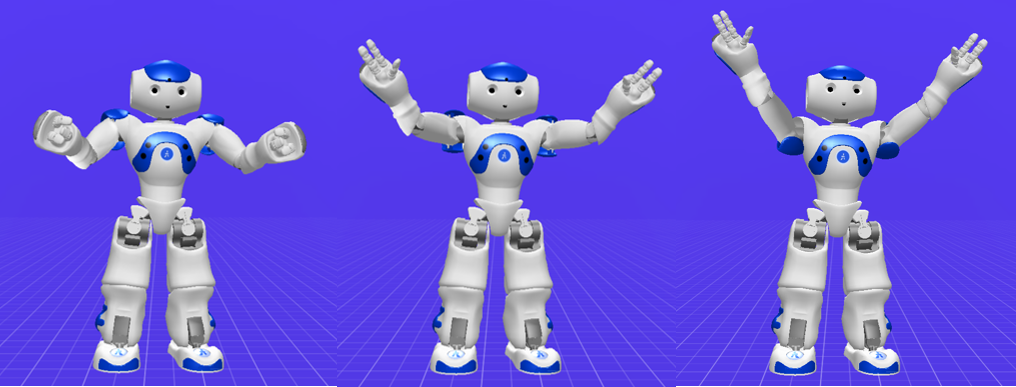
\includegraphics[width=1.0\linewidth]{./BothUpComparison}
\caption{Sample gesture ('Both Up') in the sad, neutral and happy conditions demonstrating the different in the Extent parameter across conditions. [demo video ref or footnote here?]}
\label{fig:BothUpComparison}
\end{figure}


\subsection{Speech Generation}
Cereproc's CereVoice Engine Text-to-Speech SDK [REF NEEDED HERE? OR FOOTNOTE MAYBE?] was used to create all speech for the robot. The CereVoice engine was selected because it supports a number of SSML tags for voice modification which would allow application of the SIRE framework but also offers pre-defined emotional tags for generating emotional speech. The supported SSML tags identified for mapping onto SIRE parameters are listed in Table [REF]; however for this project it was decided, providing the testing and validation of the voice yielded good results, to use the pre-determined emotional tags [WHY?? - simpler \& quicker, might use voice to generate SIRE values for gestures in future, figured it was tested and good already]. 

\begin{tabular}{|c|c|}
	\hline SIRE Parameter & Cerevoice Tag(s)\\ 
	\hline Speed & rate \\ 
	\hline Intensity & rate, duration \\ 
	\hline Regularity & break, duration \\ 
	\hline Extent & pitch range, pitch contour \\ 
	\hline 
\end{tabular}

All speech files were generated in advance of the experiment and stored as .wav files within the robots control program. 

\subsection{Choregraphe}
Implementation of the SIRE algorithm and control of the NAO was all undertaken within Softbank Robotics graphical user interface, Choregraphe. Individual gestures with SIRE parameterisation were scripted in Python and embedded in a Choregraphe box which allowed for easy slider-manipulation of each SIRE value. All other aspects of control e.g. making the robot stand, turning LEDs on and off, reading touch sensors etc. were achieved using standard Choregraphe library boxes. The final experiment Choregraphe control script is detailed in Section [REF]. 

\section{Testing \& Validation of Emotion Expression}
Three emotion recognition experiments were carried out in order to test the initial SIRE values described above. The first two tested emotion recognition in voice only and gesture only whereas the third tested the combined voice and gesture. Testing each modality independently at first allowed for validation of the CereVoice emotional SSML tags and SIRE framework. Testing the combined performance allowed for validation of the final system as intended for use in the main HRI experiment. 

[VIDEO LINK perhaps in footnote]

All three experiments were administered through an online survey in which participants were asked to watch and/or listen to a video and rate the emotional state of the robot or speaker (video screen was a simple title slide the voice only condition). The same 16 participants were recruited for experiments one and two covering the voice only and gesture only conditions; a new set of 25 participants were recruited for the combined condition. All surveys consisted of 4 samples of each condition, neutral, happy and sad, and the order of the videos was randomised for each participant. Percentage recognition results for each condition are given in table [REF]; it can be seen they are very similar to Lim et al.'s reported result of 60\%+ . 

\begin{tabular}{|c|c|}
	\hline Condition & Recognition\\ 
	\hline Voice Only & 60.4\% \\ 
	\hline Gesture Only & 68.2\% \\ 
	\hline Voice + Gesture & 65.0\% \\ 
	\hline 
\end{tabular} 

Chi-square contingency table analyses were performed to check whether the intended emotion was identified significantly more frequently than the other options in each condition. This was always found to be the case with $\chi^{2}(1,300) = 8.85 - 54.6$ and $p < 0.01 - 0.05$. [IS this reported correctly? 1 = dof in each case because comparing only 2 emotions and 300 = total number of samples?]. Contingency table analyses were also performed to check the variation in recognition and extreme choices across the voice only, gesture only and voice plus gesture conditions. Overall recognition did not vary significantly but the number of extreme emotion choices (i.e. very happy or very sad) significantly increased between the voice only and voice plus gesture conditions $\chi^{2}(1,492) = 5.66, p <0.05$. This is discussed further in Section [REF DISCUSSION SECTION]. Based on these results it was decided to leave the initial SIRE values unchanged and to use the CereVoice emotion tags only for generating the robot's speech, rather than extending the SIRE framework to include voice manipulation. 

\section{Human Robot Interaction Experiment Design}
\subsection{Interaction Context}

An imitation based robot-led exercise session was chosen to provide a contextualised HRI activity for testing the impact of affective robot communication. An imitation based activity was preferred as it inherently encourages the participant to focus on the robot's gestures; Xu et al. used a gesture imitation game for this reason \cite{xu2014robot}. However, there is psychological evidence that winning or losing at a game can influence mood, attitude and likelihood of further game participation \cite{ward1988promotional}. It was therefore decided that a game based interaction should not be used in order to avoid any unintended emotional impact on participants. 

The use of robot exercise instructors has been investigated in multiple HRI studies (e.g. \cite{fasola2010robot}, \cite{goetz2002cooperation}, \cite{gockley2006encouraging}). Specifically relevant to this project is Fasola and Mataric's work on a robotic arm exercise instructor for the elderly \cite{fasola2010robot} which essentially results in the same robot interaction as Xu et al.'s set-up \cite{xu2014robot} but contextualised as a workout rather than a game. It was therefore decided to design an arm gesture exercise session in line with Fasola and Mataric's work which used the gestures employed by Xu et al. in order to allow for maximum comparison between the results from that work and this project. 

Other work by Tapus and Mataric investigated the effect of robot personality on participant's motivation to do repetitive and monotonous stroke exercises \cite{tapus2008user}. Participants were asked to do as much of each exercise as they felt necessary and this number was recorded as a quantitative measure of motivation. Similar techniques have been employed in other HRI studies such as Nakagawa et al.'s investigation of robot touch and monotonous task motivation \cite{nakagawa2011effect} and Goetz and Kiesler's study of robot seriousness and exercise regime compliance \cite{goetz2002cooperation}. Based on this it was decided that the robot-led exercise session should consist of one mandatory gesture set (in order to provide an opportunity for emotion contagion to occur) followed by a series of voluntary rounds, the number of which completed by each participant offering a quantitative measure of their motivation. An overview of the interaction flow can be seen in Figure \ref{fig:SimpleInteractionFlow}.

\begin{figure}
\centering
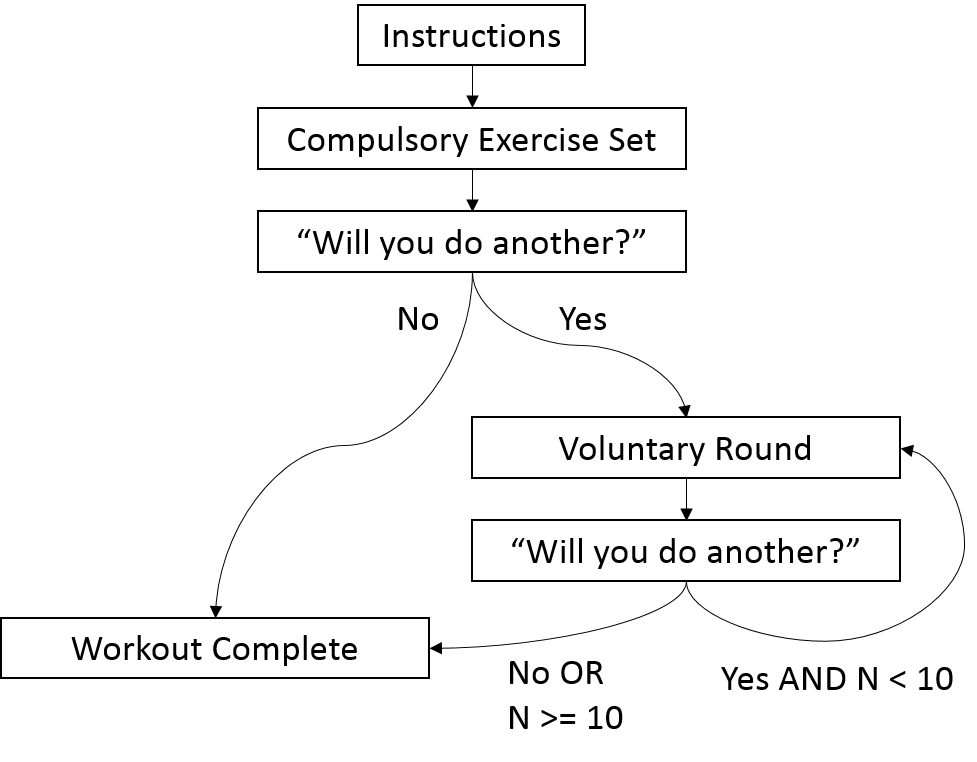
\includegraphics[width=0.7\linewidth]{./SimpleInteractionFlow}
\caption{}
\label{fig:SimpleInteractionFlow}
\end{figure}

\subsection{Robot Script}

The NAO was programmed firstly to stand, read out the initial instructions and ask the participant to touch its head if they were ready to begin; at this point the eyes turned green to indicate it was waiting for a response. Once the robot sensed a head touch it proceeded to go through the mandatory round, at the end of which it asked whether the participant would like to do another round, to touch the head for yes or foot for no, and again the eyes turned green. If the participant pressed the head then the robot went through another round of exercise and repeated the question again. If the participant pressed the foot then the robot thanked them for exercising with it and sat down. Physical touch rather than speech recognition was used for this continuation check in order to reduce the likelihood of incorrect classifications which would nullify the quantitative measure of voluntary exercise rounds. The number of voluntary rounds was capped at 10 using a for loop; when this number was reached the robot told the participant they had done the maximum amount of exercise for today and sat down as in the foot touch situation. Figure \ref{fig:ChoregrapheFlow2} shows the Choregraphe block diagram used to control the NAO, representing the final implementation of the simple control flow shown in Figure \ref{fig:SimpleInteractionFlow}.

\begin{figure}
\centering
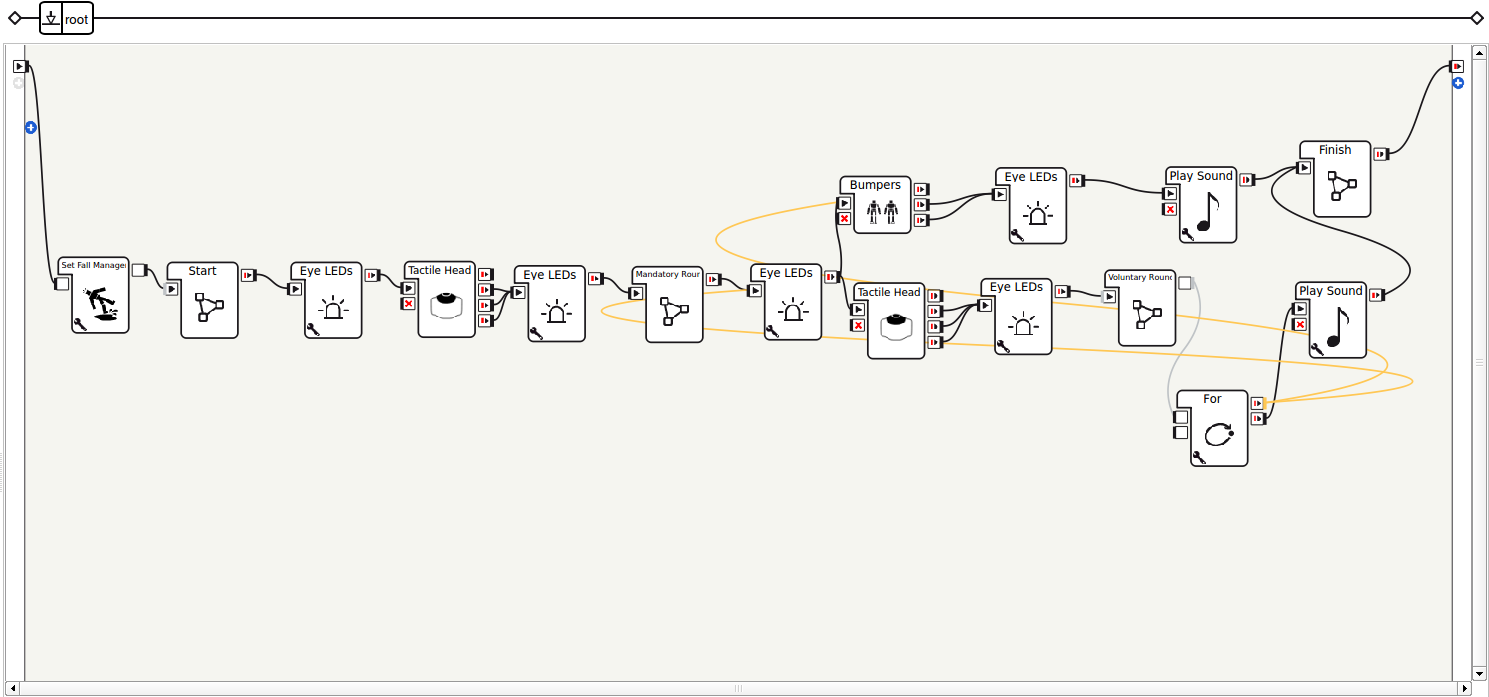
\includegraphics[width=1.0\linewidth]{./ChoregrapheFlow2}
\caption{}
\label{fig:ChoregrapheFlow2}
\end{figure}

Each round of exercise consisted of four gestures followed by a verbal confirmation that another round had been completed and a positive encouragement; this is depicted in Figure \ref{fig:ExerciseRound}. The gestures were taken directly from those used in Xu et al.'s imitation game \cite{xu2014robot} and are listed in Table [REF], which also contains the list of encouragements used. For gestures involving the left and right the instructions were reversed to the physical action such that participants had to mirror the robot; for example when the robot said "put your right arm up" it actually raised its left arm, which participants mirrored by raising their right arm. The mandatory round of exercise was the same for all participants; each voluntary round was chosen randomly in real time from ten alternative, pre-determined options using a random number generator. The gesture and encouragement combinations used in each of the ten options were also generated randomly prior to scripting the robot's control programme. The robot did not monitor the participants' performance in any way. 

\begin{figure}
\centering
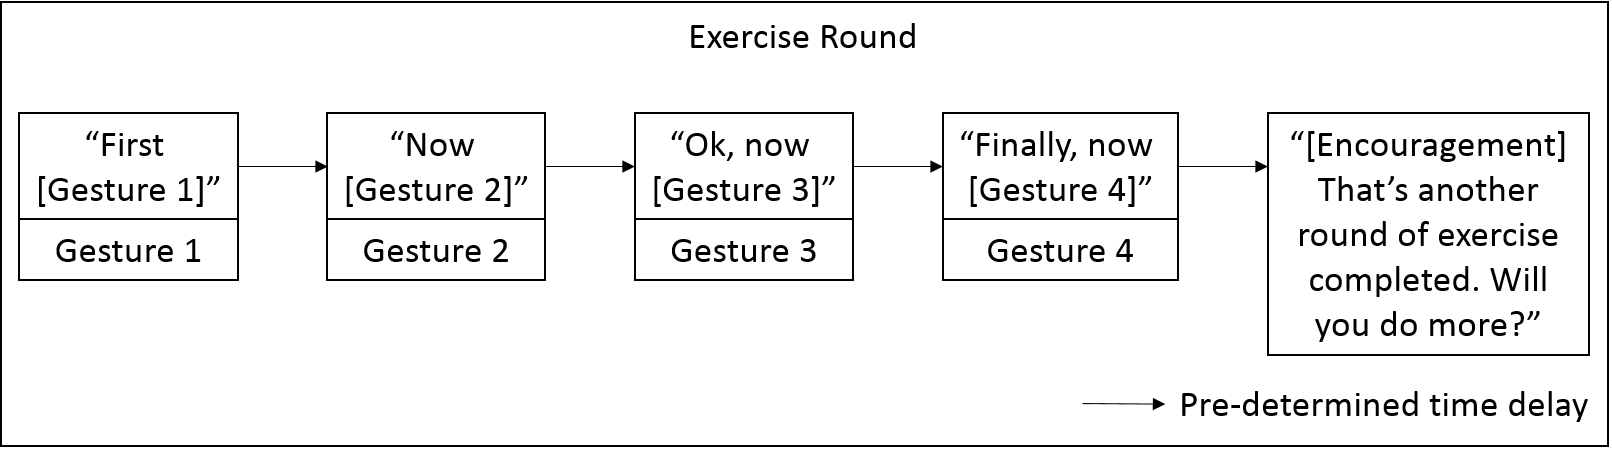
\includegraphics[width=1\linewidth]{./ExerciseRound}
\caption{}
\label{fig:ExerciseRound}
\end{figure}

\begin{tabular}{|l|p{7cm}|}
\hline Gesture Instructions & put your right arm up \newline put your right arm down \newline put your left arm up \newline put your left arm down \newline put both arms up \newline put both arms down \newline put your right arm up and left arm down \newline put your left arm up and right arm down \\ 
\hline Encouragement & great, well done \newline awesome \newline you're doing really well \newline fantastic \newline excellent \newline nice \newline good job \\ 
\hline 
\end{tabular} 

\subsection{Hypotheses \& Measures}
The four key hypotheses to be investigated in this project are as follows:

\begin{itemize}
	\item[H1] Participants in the valenced conditions will demonstrate an emotional state of matching valence after interacting with the robot, (i.e. emotion contagion will occur)
	\item[H2] Participants will recognise the intended emotional state of the robot when interacting with it
	\item[H3] Emotion expression will have an impact on human motivation and enjoyment 
	\item[H4] Emotion expression will have an impact on robot perception
\end{itemize}

H1 describes the expectation that some evidence for robot to human emotion contagion will be found. This is based on the fact that Xu et al. found some evidence for contagion during their robot-led gesture imitation game on which this project draws heavily \cite{xu2014robot}. H2 states that participants will be able to recognise whether they are working with the sad, happy or neutral robot and is based on the results of the pre-test work described in Section [REF] as well as Xu et al.'s and Lim's positive emotion recognition results \cite{xu2014robot} \cite{lim2011converting}. 

H3 and H4 describe the expectation that the use of affective movement and speech in the exercises session context will have an impact on people's behaviour, enjoyment and perception of the robot. This is based firstly on the human psychology literature discussed in Section [REF lit review], e.g. the observation that people may take different amounts of drink from a jug depending on whether it is offered by a smiling face or frowning face. In addition, it is expected based on HRI studies which have demonstrated how changing a robot's behaviour can change participant behaviour and perception; for example Nakagawa et al.'s active touch and motivation study or Chidambaram et al.'s communication cues and persuasion study.

Overall these hypotheses can be grouped under two key features of interest; robot to human emotion contagion and the impact of affective communication on HRI. The experimental measures relevant to each area of interest and the specific hypotheses they relate to are listed in Table [REF].  

\begin{tabular}{|l|p{7cm}|p{3.8cm}|}
\hline Feature of Interest & Related Measures & Relevant Hypotheses \\ 
\hline Emotion Contagion & Word completion task \newline Emotional state (of robot and self) & H1 \newline H1 \& H2 \\ 
\hline Impact on HRI & Number of exercise rounds voluntarily completed \newline Enjoyment Likert scale \newline Reason for stopping Likert scale \newline Perceived usefulness Likert scale \newline Selected Godspeed Questions \newline Open feedback/comments &  H3 \newline \newline H3 \newline H3 \newline H4 \newline H4 \newline H4 \\
\hline 
\end{tabular} 

It was decided to measure the emotional state of the participants using both an implicit and explicit measure. As discussed in Section [REF lit reivew], some emotion contagion effects in humans may be subconscious and so it seems sensible to also include an implicit mood measure in the surveying of participants. Measuring mood with both explicit and implicit measures also allows for a comparison between participants conscious and subconscious feelings. Previous HRI studies have typically measured subconcious emotional state using video coding analysis to look for visual emotional cues such as smiles and laughter [REFs], however this was deemed impractical for this project for two reasons. Firstly, video coding is a timely procedure which requires individual analysis of each participant; this is particularly an issue given the large number of participants involved in this study. Secondly it was hypothesised that the use of video recording equipment and participants' knowledge that they were being filmed may affect the number of voluntary exercise rounds they chose to complete [do i need to ref why i think that?]. Therefore, a participant task based approach was preferred. A word completion test was chosen for this purpose and is discussed in more detail below. 

Quantitatively measuring participant motivation was one of the key aims of this project; as discussed in Section [REF interaction context] the exercise session with voluntary rounds context was derived in part directly to achieve this. The use of voluntary exercise rounds as a quantitative measure is inspired by previous studies which have used voluntary participation as a quantitative measure (e.g. \cite{gockley2006encouraging}, \cite{nakagawa2011effect}) as discussed in detail in Sections [REF lit review and interaction context]. 

A number of Likert style questions were derived in order to evaluate differences in participants' experience and robot perception across the different emotional conditions. Firstly participants were asked how much they enjoyed working out the robot. Secondly, based on questions asked by Gockley and Mataric, participants were asked whether they stopped more due to boredom or tiredness and how useful the robot was in getting them to exercise \cite{gockley2006encouraging}. A number of relevant questions taken from The Godspeed Questionnaire Series, a standardised set of HRI questionnaires \cite{bartneck2009measurement} were also included in the survey. Finally participants were asked to leave any additional thoughts, comments or feedback in an open text box question. [FULL SURVEY IN APPENDIX?]

\subsubsection{Word Completion Test}

Word completion tests require the participant to complete a word stem, a word with one or more missing letters, which has multiple potential completions. In HRI studies, such tests have typically been used measure death thought accessibility linked to the Uncanney Valley effect \cite{koschate2016overcoming}; but they have also been used in human psychology studies in order to measure emotional state e.g. \cite{dewall2007terror}. Other implicit mood measures considered include a memory recall test \cite{seibert1991irrelevant} or creative task performance \cite{isen1987positive}. Creative task performance was disregarded because it only tests for positive mood, meaning an alternative test would have been required for participants in the negative condition. In \cite{seibert1991irrelevant} emotional states were induced in participants using strongly valenced statements and in their discussion of the measured impact on memory recall the authors state memory might be affected due to an increase in irrelevant thoughts linked to these statements. It is not clear how well the memory measure would therefore work on more subtle emotional manipulation.

A word stem list was generated using Bradley and Lang's Affective Norms for English Words (ANEW): Instruction Manual and Affective Ratings \cite{bradley1999affective}. Firstly all words with a valence greater than 7 (positive), less than 3 (negative) and exactly 5 (neutral) were identified. Possible word stems and alternative completions were then considered for each of the valenced words to find word stems which had one valenced completion (positive or negative only) and one or more neutral completions. For the neutral words word stems with only neutral completions were selected. Finally the word frequencies of these alternative completions were compared and all word stems with a difference greater than 1 in any possible completion were discarded. 12 neutral, 6 positive and 6 negative words were selected from the remaining pool to generate an initial word list. 

A pretest of 8 subjects was then carried out to examine completion frequencies of the valenced words in a relatively neutral context. Valenced word stems which were completed by more than 50\% of participants were discarded and replaced with others from the pool described above. The final valenced word stems and possible completions are given below; the list of neutral filler words can be found in [REF appendix]. All participants completed the entire word list of negative, positive and neutral word stems. 

[Something about how proper validation would work and that this is further work to make the tool a more validated measure etc] 

\begin{tabular}{|c|c|c|}
\hline Word Stem & Valenced Completion & Neutral Completion(s) \\ 
\hline \_ I L L E R & KILLER & FILLER \\ 
\hline \_ R I M & GRIM & TRIM, PRIM, BRIM \\ 
\hline S H \_ N & SHUN & SHIN \\ 
\hline W A \_ P & WASP & WARP \\ 
\hline C R E E \_ & CREEP & CREED \\ 
\hline \_ A S T Y & NASTY & TASTY \\ 
\hline 
\end{tabular} 

\begin{tabular}{|c|c|c|}
\hline Word Stem & Valenced Completion & Neutral Completion(s) \\ 
\hline J O \_ & JOY & JOG, JOT \\ 
\hline D \_ N \_ E & DANCE & DENSE \\ 
\hline \_ I F T & GIFT & LIFT, RIFT \\ 
\hline B I \_ D & BIRD & BIND \\ 
\hline B R A \_ E & BRAVE & BRACE, BRAKE \\ 
\hline \_ A I R & FAIR & PAIR, LAIR, HAIR \\ 
\hline 
\end{tabular} 

\subsection{Experimental Procedure}
A total of 62 participants (18 male and 44 female) aged between 21 and 60 (Mean = 31.7 SD = 8.72) were recruited for the experiment and randomly assigned to one of the three conditions resulting in 21 subjects in the happy and neutral conditions and 20 subjects in the sad condition. The quantitative data for one subject in the happy condition was discarded due to a fire alarm disrupting the experiment. Participants were offered a $�5$ Amazon voucher as compensation for taking part in the experiment. 

Participants were first asked to read through an experiment information sheet which stated that the NAO was programmed to guide them through an arm exercise session typically used by older adults and the disabled to keep fit. It was explained that each round of exercise consisted of 4 gestures and that the first round of exercise was mandatory, but after that NAO would ask the participant if they wanted to continue or stop and that they could stop exercising whenever they wanted to; this was highlighted in bold text. 

A demo was then given to show the participants what to expect and how to safely interact with the robot in terms of touching the head or foot to indicate they wanted to continue or end the exercise session respectively. At this point it was verbally pointed out again to the participants that all exercise rounds after the first were voluntary and they could stop at any time. The experimenter than launched the main experiment script and left the room once the robot was seen to be working correctly, returning when the exercise session was complete, either because the participant chose to end the session or the maximum number of rounds was reached.

Once the exercise session was complete participants were asked to complete an online survey containing the word completion task, all Likert and Godspeed questions and robot/self emotional state questions. Participants were then asked to read a debrief sheet which explained the underlying study of affective communication and its impact on HRI with a note not to discuss this with any other potential participants until after they had also completed the experiment. Participants were then given a final chance to ask any questions about or discuss the research further with a note made of any additional qualitative feedback. 

\chapter{Results}

\section{Robot to Human Emotion Contagion}
\subsection{Robot Emotion Recognition}
Figure \ref{fig:RobotMood} shows participants' perception of the robot's emotional state across conditions; essentially a manipulation check of whether the intended emotions were recognised. Clearly this was not the case. Almost all participants judged the robot to be either neutral or happy with roughly an equal split between the two. Interestingly the largest difference was in the happy condition, where the robot was judged to be neutral more often than happy, however [analysis] showed this wasn't significant.  

\begin{figure}
	\centering
	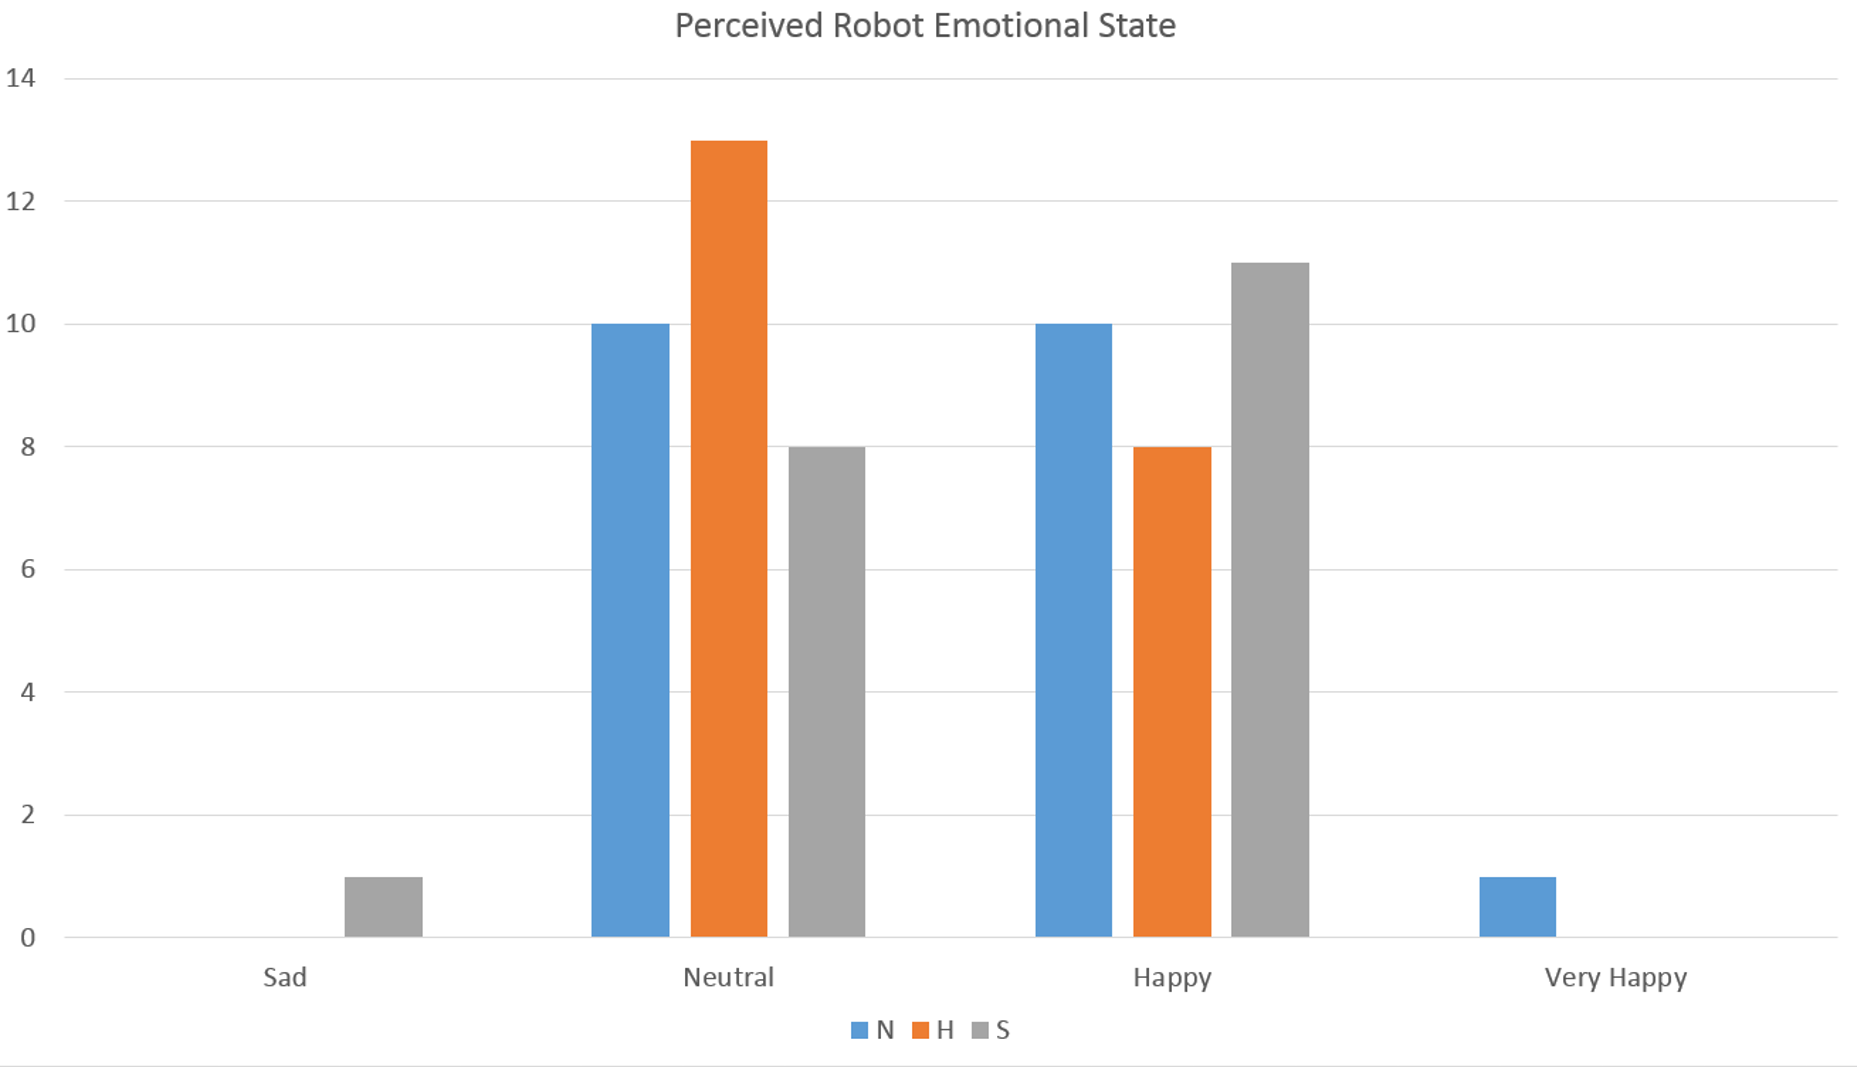
\includegraphics[width=\linewidth]{RobotMood}
	\caption{}
	\label{fig:RobotMood}
\end{figure}

\subsection{Human Mood Measures}
The mean number of positive, negative and total emotive word completions per participant are listed in Table[REF]. One way ANOVA tests with the number of positive, negative and total emotive word completions were carried out in order to check for differences across the three emotion conditions. It can be seen in Table [REF] that the number of emotive completions did increase between the neutral and emotive conditions; however the ANOVA analysis yielded no significant difference. In order to account for the Figure \ref{fig:SelfAssessedMood} shows the number of participants that selected each of the possible emotional state descriptor faces to describe their own emotional state when interaction with the robot; the similarity in response across conditions is clear and therefore no additional statistical analysis was undertaken. In all conditions the majority of participants indicated they were happy and no participants indicated they were sad or very sad whilst interacting with the robot. 

\begin{tabular}{|c|c|c|c|}
	\hline & M(Positive) & M(Negative) & M(Total) \\ 
	\hline Neutral & 1.19 & 1.05 & 2.24\\ 
	\hline Happy & 1.62 & 1.05 & 2.67 \\ 
	\hline Sad & 1.43 & 1.24 & 2.67 \\ 
	\hline 
\end{tabular} 

\begin{figure}
\centering
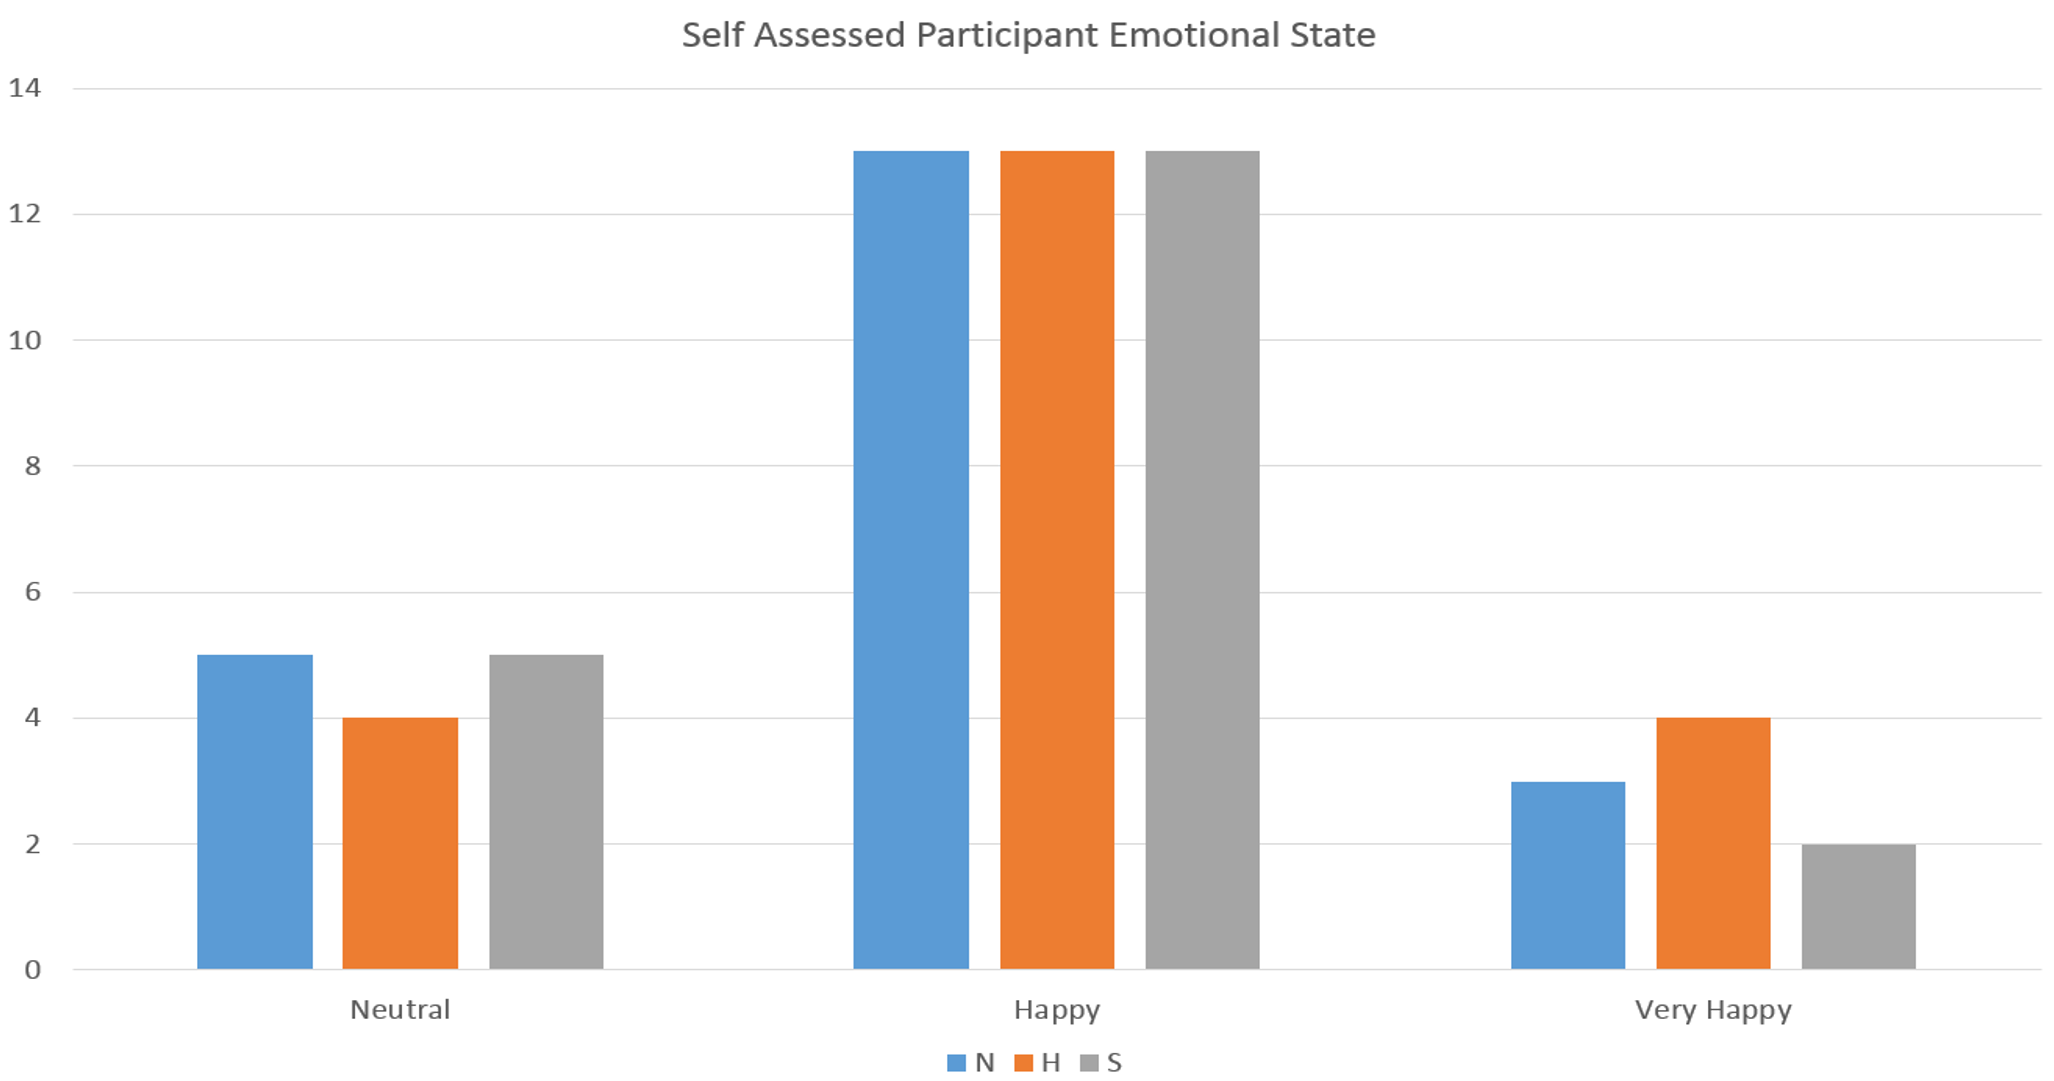
\includegraphics[width=\linewidth]{SelfAssessedMood}
\caption{}
\label{fig:SelfAssessedMood}
\end{figure}

\section{Impact of Affective Communication on HRI}
\subsection{Voluntary Exercise Rounds \& Closed Survey Questions}
The mean number of voluntary rounds undertaken by participants in each condition is listed in Table [REF]. This data suggests that people exercised less with the happy robot however a one way ANOVA analysis yielded no significant difference between conditions (p = 0.14). 

\begin{tabular}{|c|c|}
	\hline & Average Rounds\\ 
	\hline Neutral & 8.67 \\ 
	\hline Happy & 7.33 \\ 
	\hline Sad & 8.15 \\ 
	\hline 
\end{tabular} 

One way ANOVA analyses were also carried out for each of the Likert and semantic difference scale survey questions; no significant differences were found in the responses to any question across the three emotion conditions. 

\subsection{Open Question Qualitative Data}
[Qualitative data from open ended question at end - look at use of adjectives across conditions, note people saying emotion questions were difficult as they 'knew it couldn't have emotions']

\chapter{Discussion}

Not sure where this fits but definitely want some discussion on people's expectations and how this changes their judgements i.e. the robot must be neutral because it is a robot and robots dont have emotions (qualitative data which is also discussed in 'how robots should give advice' paper as a reason for the same behaviour done by a robot and human leading to different responses). 

\section{Emotion Recognition in Robot Gesture and Voice}
\begin{itemize}
	\item perceived extremity increased by use of gestures - relevant to telepresence etc
	\item why was emotion recognised correctly in pre test but not exercise experiment? Relative difference? How does this contrast to Lim's result? Can offer quite a lot of discussion on this
	\item Literature suggests emotion should be recognisable in semantic free motion and voice so why didn't I get that? Did all literature reviewed studies ask people specifically what emotion they thought the robot had? Were their studies 'hidden' under a context (i.e. mine was set up as an exercise experiment?) because if so that's quite an interesting result which challenges the existing literatue and says actually people need to be expecting the emotional aspect for it to work, which ties in with the fact my recognition experiments got good results - yeah actually this is pretty big result the fact that asking people to look for the emotion got good results but implicitly using them returned nothing. That's really important for future work and for emotional robotics in general. 
	\item comparison to Xu et al - maybe to do with use of emoji faces compared to asking for mood valence or something? as in maybe the emojis were too much? have a look at the actual types of questions asked for measuring perceived mood there could be some conflict there perhaps which means i didn't pick up any effect where i should have
	\item could xu's result be wrong i.e. participants did indeed have worse moods in bad condition but just because the task was harder?
	\item Xu had huge head movements and much less spoken information - could be that for me the use of any encouragement at all overwrote the subtlety of movement and tone of voice
\end{itemize}

\section{Robot to Human Emotion Contagion}

\section{Impact of Affective Communication on HRI}
Perception and motivation - liket scale Q's and voluntary rounds completed

Might want to refer to \cite{kennedy2016social} here as they too expected to see an impact of something (immediacy) on a measure (learning) and didn't. 

\chapter{Conclusions}

Perhaps robot needs to be more explicit about it's emotional state in order for emotion recognition to occur, at least if the situation is one in which emotions wouldn't really be expected. 

\section{Further Work}

A multiple interaction experiment whereby the participant is going to see the different emotional states of the robot. 

An experiment where the robot is explicit about its emotional state to see impact on persuasiveness and contagion - could almost do exactly the same experiment but with explicit emotional discussion at start or some context for that or something.

\bibliographystyle{unsrt}
\bibliography{MyReading}

\end{document}